\section{Modelagem matemática para roteirização}\label{sec:matemática}
Problemas de roteirização de ônibus podem ser resolvidos por modelagem, seguida de implementação em ambiente computacional. Para a compreensão dos modelos, é necessário entender conceitos básicos de teoria dos grafos. Para entender como a resolução dos problemas funciona, um aprofundamento matemático em álgebra linear é importante.

O conteúdo de grafos desta seção toma como base os materiais de \textcite{PRESTES:20,FEOFILOFF:11}. Já o conteúdo de álgebra linear é baseado, principalmente, em \textcite{BAZARAA:10,BERTSIMAS:97,FERRIS:07}.

\subsection{Grafos e dígrafos simples}
\begin{mydef}[Grafo simples]
    Um \emph{grafo simples} $G = (\mcal{V}, \mcal{A})$ é uma estrutura discreta formada por um conjunto de vértices $\mcal{V}$, com $\mcal{V} \neq \emptyset$, e um conjunto de arestas $\mcal{A} \subseteq \mcal{P}(\mcal{V})$, com $\mcal{P}(\mcal{V}) = \{\{x,y\}\mid x \neq y \land x,y \in \mcal{V}\}$. No máximo uma aresta é associada a cada par de vértices.
\end{mydef}

Devido à natureza dos problemas de roteirização, boa parte dos autores trata os pontos a serem visitados como vértices, com os deslocamentos entre pontos sendo representados por arestas. A \cref{fig:grafo simples} ilustra um grafo da forma $G = (\mcal{V}, \mcal{A})$.

\begin{figure}[h]
\centering
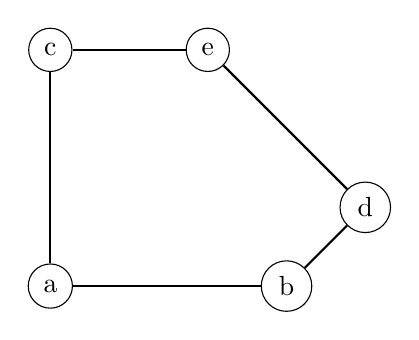
\begin{tikzpicture}
\tikzstyle{vx} = [circle,draw=black] %vertex
\tikzstyle{ue} = [-,thick] %undirected edge
\node[vx](va)at(0,0){a};
\node[vx](vb)at(3,0){b};
\node[vx](vc)at(0,3){c};
\node[vx](vd)at(4,1){d};
\node[vx](ve)at(2,3){e};
\draw[ue](va)--(vb);
\draw[ue](vb)--(vd);
\draw[ue](vd)--(ve);
\draw[ue](ve)--(vc);
\draw[ue](vc)--(va);
\end{tikzpicture}
\caption{}\label{fig:grafo simples}
\end{figure}

Quando uma aresta conecta dois vértices $a$ e $b$, diz-se que ela \emph{incide} sobre $a$ e $b$. A definição de grafo simples não especifica um sentido de conexão entre os pontos. Para situações em que o sentido importa, recorre-se a \emph{dígrafos simples}.

\begin{mydef}[Dígrafo simples]
    Um \emph{dígrafo simples}, ou \emph{grafo orientado}, $D = (\mcal{V}_d, \mcal{A}_d)$ é um grafo com conjunto de vértices $\mcal{V}_d$ e conjunto de arestas $\mcal{A}_d \subseteq \mcal{P}_d(\mcal{V})$, com $\mcal{P}_d(\mcal{V}) = \{(x,y) \mid x \neq y \land x,y \in \mcal{V}_d\}$. Para cada par de vértices $x$ e $y$, podem existir no máximo duas arestas relacionando os vértices. Neste caso, uma deve ser $(x,y)$ e a outra deve ser $(y,x)$.
\end{mydef}

É comum referir-se às arestas de um dígrafo como \emph{arcos}. Os arcos são representados por pares ordenados porque a ordem de deslocamento entre vértices importa. Assim, $(x,y)$ indica deslocamento com origem em $x$ e destino em $y$, e $(y,x)$ indica deslocamento na direção contrária.

A \cref{fig:dígrafo simples} ilustra um dígrafo simples. Na representação visual, a ponta da flecha do arco indica o destino, e a outra extremidade indica a origem.

\begin{figure}[h]
\centering
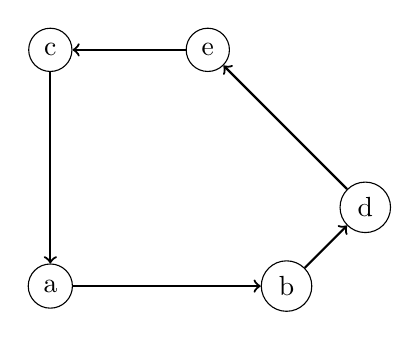
\begin{tikzpicture}
\tikzstyle{vx} = [circle,draw=black] %vertex
\tikzstyle{de} = [->,thick] %directed edge
\node[vx](va)at(0,0){a};
\node[vx](vb)at(3,0){b};
\node[vx](vc)at(0,3){c};
\node[vx](vd)at(4,1){d};
\node[vx](ve)at(2,3){e};
\draw[de](va)--(vb);
\draw[de](vb)--(vd);
\draw[de](vd)--(ve);
\draw[de](ve)--(vc);
\draw[de](vc)--(va);
\end{tikzpicture}
\caption{}\label{fig:dígrafo simples}
\end{figure}

\begin{mydef}[Subgrafo]
    Um grafo $G_1 = (\mcal{V}_1, \mcal{A}_1)$ é um \emph{subgrafo} de $G_2 = (\mcal{V}_2, \mcal{A}_2)$, denotado $G_1 \subseteq G_2$, se e só se $\mcal{V}_1 \subseteq \mcal{V}_2$ e $\mcal{A}_1 \subseteq \mcal{A}_2$. Neste caso, $G_1$ é \emph{supergrafo} de $G_1$.
\end{mydef}

\begin{mydef}[Subgrafo induzido por vértices]
    Sejam $G = (\mcal{V}, \mcal{A})$ um grafo e $S_v \subseteq \mcal{V}$ um subconjunto não-vazio. Dizemos que um subgrafo de $G$ é \emph{induzido} por $S_v$ (denotado por $G[S_v]$) se seu conjunto de vértices é $S_v$ e seu conjunto de arestas é composto por todas as arestas de $G$ que possuem ambas as extremidades em $S_v$. 
\end{mydef}

As \cref{fig:subgrafo induzido A,fig:subgrafo induzido B} ilustram um grafo e um de seus subgrafos, respectivamente.

\begin{figure}
\centering
\begin{subfigure}{.5\textwidth}
  \centering
  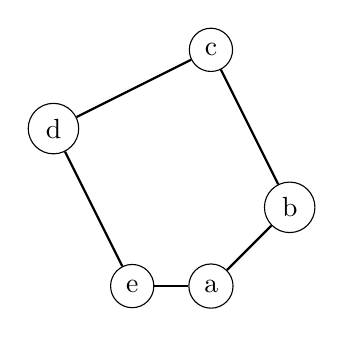
\begin{tikzpicture}
    \tikzstyle{vx} = [circle,draw=black] %vertex
    \tikzstyle{ue} = [-,thick] %undirected edge
    \node[vx](va)at(0,0){a};
    \node[vx](vb)at(1,1){b};
    \node[vx](vc)at(0,3){c};
    \node[vx](vd)at(-2,2){d};
    \node[vx](ve)at(-1,0){e};
    \draw[ue](va)--(vb);
    \draw[ue](vb)--(vc);
    \draw[ue](vc)--(vd);
    \draw[ue](vd)--(ve);
    \draw[ue](ve)--(va);
  \end{tikzpicture}
  \caption{Grafo $G = (V, A)$.}\label{fig:subgrafo induzido A}
\end{subfigure}%
\begin{subfigure}{.5\textwidth}
  \centering
  \begin{tikzpicture}
    \tikzstyle{vx} = [circle,draw=black] %vertex
    \tikzstyle{ue} = [-,thick] %undirected edge
    \node[vx](va)at(0,0){a};
    \node[vx](vb)at(1,1){b};
    \node[vx](vd)at(-2,2){d};
    \draw[ue](va)--(vb);
  \end{tikzpicture}
  \caption{Subgrafo induzido $G[\{a, b, d\}]$.}\label{fig:subgrafo induzido B}
\end{subfigure}
\label{fig:subgrafo induzido por vértice}
\end{figure}

\subsection{Conexões entre vértices}
\begin{mydef}[Vértices vizinhos]
    Dado um grafo simples $G = (\mcal{V}, \mcal{A})$, dizemos que dois vértices $v_i,v_j \in \mcal{V}$ são \emph{vizinhos} se existe aresta $\{v_i,v_j\} \in \mcal{A}$. No caso de um dígrafo simples $D = (\mcal{V}_d, \mcal{A}_d)$, dois vértices são vizinhos se existe arco $(v_i,v_j) \in \mcal{A}_d$ ou $(v_j,v_i) \in \mcal{A}_d$. Em ambos os casos, estamos assumindo que $v_i \neq v_j$.
\end{mydef}

A \emph{função de vizinhança}, $\tau : V \rightarrow 2^V$, de um grafo simples $G = (\mcal{V}, \mcal{A})$, é

\begin{equation}
    \tau(v) = \{w \mid \{v, w\} \in \mcal{A}\},
\end{equation}
em que $2^V$ é o conjunto potência de $V$.

Já para um dígrafo simples $D = (\mcal{V}_d, \mcal{A}_d)$, existem duas funções de vizinhança: a \emph{direta} ($\tau^+ : \mcal{V} \rightarrow 2^{\mcal{V}_d}$) e a \emph{inversa} ($\tau^- : \mcal{V} \rightarrow 2^{\mcal{V}_d}$), definidas, respectivamente, a seguir.

\begin{equation}
    \tau^+(v) = \{w \mid (v, w) \in \mcal{A}_d\}
\end{equation}
e
\begin{equation}
    \tau^-(v) = \{w \mid (w, v) \in \mcal{A}_d\}.
\end{equation}

A função de vizinhança serve como base para o conceito de \emph{grau}.

\begin{mydef}[Grau de um vértice]
    Para um grafo simples $G = (\mcal{V}, \mcal{A})$, o \emph{grau} de um vértice $v$, denotado por $d(v)$, é igual ao seu número de vizinhos. Ou seja, $d(v) = |\tau(v)|$.

    No caso de um dígrafo simples $D = (\mcal{V}_d, \mcal{A}_d)$, o \emph{grau de entrada} $d^-(v)$ e o \emph{grau de saída} $d^+(v)$ são definidos, respectivamente, como $d^-(v) = |\tau^-(v)|$ e $d^+(v) = |\tau^+(v)|$.
\end{mydef}

Representaremos o maior e o menor grau de todos os vértices em um grafo $G$, respectivamente, como

\begin{equation}
    \Delta(G) = \max_{v \in \mcal{V}} d(v)
\end{equation}
e
\begin{equation}
    \delta(G) = \min_{v \in \mcal{V}} d(v).
\end{equation}

As incidências sobre os vértices de um grafo são passíveis de representação matricial.

\begin{mydef}[Matriz de adjacência]
    Para um grafo simples $G = (\mcal{V}, \mcal{A})$, com $\mcal{V} = \{v_1,\ldots,v_n\}$, a \emph{matriz de adjacência}, $M$, é uma matriz $n \times n$ simétrica cujos elementos obedecem à seguinte definição:

    \begin{equation}
        m_{ij} = 
        \begin{cases}
            0 \text{, se } v_i = v_j \text{ ou se } v_i \text{ não é adjacente a } v_j\\
            1 \text{, se } v_i \text{ é adjacente a } v_j.
        \end{cases}
    \end{equation}

    No caso de um dígrafo simples $D = (\mcal{V}_d, \mcal{A}_d)$ com $\mcal{V} = \{v_1,\ldots,v_n\}$, a matriz de adjacência, $A$, não necessariamente é simétrica, e seus elementos são definidos como:

    \begin{equation}
        a_{ij} = 
        \begin{cases}
            0 \text{, se } v_i = v_j \text{ ou se } v_i \text{ não é origem de um arco que tem destino em } v_j\\
            1 \text{, se } v_i \text{ é origem de um arco que tem destino em } v_j.
        \end{cases}
    \end{equation}
\end{mydef}

\begin{mydef}[Ciclo]
    Em um grafo, um \emph{ciclo} a partir de $v$ é uma sequência alternada de vértices e arestas $v = v_0, a_1, v_1, a_2, v_2, \ldots, a_n, v_n = v$ que começa e termina em $v$, com todos os vértices e arestas distintos, exceto $v_0$ e $v_n$, e com cada aresta $a_i$ incidente aos vértices $v_{i-1}$ e $v_i$.
\end{mydef}

Chamamos de \emph{cintura} o menor ciclo em um grafo $G$, denotado por $g(G)$, e de \emph{circunferência} o seu maior ciclo, denotado por $c(G)$. Um ciclo com $n$ vértices distintos precisa de $n$ arestas conectando os vértices. O número de vértices em um ciclo é conhecido como \emph{comprimento} do ciclo.

\begin{mydef}[Ciclo hamiltoniano]
    Um \emph{ciclo hamiltoniano}, ou \emph{ciclo de espalhamento}, é um ciclo no qual estão inclusos todos os vértices do grafo.
\end{mydef}

\begin{mydef}[Grafo e dígrafo hamiltonianos]
    Um grafo ou dígrafo é hamiltoniano se ele possui um ciclo hamiltoniano.
\end{mydef}

\subsection{O problema do caixeiro viajante}\label{sec:PCV}
O problema do caixeiro viajante (PCV) é o problema de roteirização de formulação mais simples. A descrição informal feita por \textcite{SAIYED:12} estabelece que

\begin{displayquote}
    O problema do caixeiro viajante envolve um vendedor que precisa passar por um conjunto de cidades tomando o caminho mais curto possível e visitando todas as cidades apenas uma vez, e não menos que uma vez, e retornando ao ponto de partida.\footnote{The traveling salesman problem involves a salesman who must make a tour of a number of cities using the shortest path available and visit each city exactly once and only once and return to the original starting point.}
\end{displayquote}

Seja $G = (\mcal{V}, \mcal{A})$ um grafo, em que $\mcal{V}$ é o conjunto de vértices a visitar e $\mcal{A}$ é o conjunto de arestas que incidem sobre os vértices entre os quais ocorre deslocamento. O PCV pode ser interpretado como o problema de determinação de uma sequência de vértices e arestas, com começo e fim num mesmo vértice e grau 2 para todos os vértices, formando um ciclo hamiltoniano \cite{ZAMBITO:06}.

Em geral, o PCV é modelado como um problema cujo objetivo é

\begin{equation}
    \min\sum_{i,j \in \mcal{V}}{x_{ij}c_{ij}},
\end{equation}
em que $c_{ij}$ são coeficientes de custo associados ao deslocamento entre os vértices $v_i$ e $v_j$, e $x_{ij}$ são variáveis que definem se ocorre deslocamento entre os vértices $v_i$ e $v_j$. As matrizes $C = [c_{ij}]$ e $X = [x_{ij}]$, que reúnem estes elementos, são chamadas, respectivamente, de matriz de custos e matriz de adjacência.

\begin{mydef}[Matriz simétrica]
    Uma matriz quadrada $A = [a_{ij}]$ é dita \emph{simétrica} quando $a_{ij} = a_{ji}, \forall i, j$.
\end{mydef}

Dizemos que o PCV é simétrico ou não dependendo da simetria da matriz de custos. \textcite{DANTZIG:54}, por exemplo, consideram que um PCV assimétrico requeira as famílias de restrições

\begin{align}
    \sum_{i\in\mcal{V}}x_{ij} = 1,\ & \forall j \in \mcal{V}, \label[constraint]{eq:restrição ida dfj assimétrico}\\
    \sum_{j\in\mcal{V}}x_{ij} = 1,\ & \forall i \in \mcal{V}, \label[constraint]{eq:restrição volta dfj assimétrico}
\end{align}
em que as \cref{eq:restrição ida dfj assimétrico,eq:restrição volta dfj assimétrico} garantem que a cada ponto se chegue e de cada ponto se saia uma única vez, respectivamente, com $x_{ij} \in \{0,1\}$, com 1 representando a existência de deslocamento de $v_i$ até $v_j$ e 0 representando a ausência de deslocamento neste sentido. Neste caso, a matriz de adjacência define um dígrafo.

Para o caso simétrico, os autores definem a família de restrições

\begin{align}
    \sum_{j \in \mcal{V}}x_{ij} = 2,\ \forall i \in \mcal{V}.
\end{align}

Além de implicar formulações mais simples, o PCV simétrico tem metade do número de soluções possíveis do assimétrico, por não importar o sentido de deslocamento de um ponto a outro.

As restrições acima não impedem que ocorram soluções em que não é formado ciclo hamiltoniano, como X = I\footnote{Quando $x_{ii} = 1$, $i \in \mcal{V}$, diz-se que o vértice $v_i$ apresenta um \emph{laço}. Neste caso, a solução encontrada é um \emph{pseudografo}.}, ilustrada na \cref{fig:PCV laços}, ou qualquer outra solução que envolva a formação de ciclos de menor comprimento, que chamamos de \emph{subciclos}, como exemplificado na \cref{fig:PCV subciclos}.

\begin{figure}[h]
\begin{subfigure}{.4\textwidth}
\centering
\begin{tikzpicture}
\tikzstyle{vx} = [circle,draw=black] %vertex
\tikzstyle{de} = [-,thick] %directed edge
\node[vx](va)at(0,0){1};
\node[vx](vb)at(3,0){2};
\node[vx](vc)at(0,3){3};
\node[vx](vd)at(4,1){4};
\node[vx](ve)at(2,3){5};
\path(va) edge [loop above] node{} (va);
\path(vb) edge [loop above] node{} (vb);
\path(vc) edge [loop above] node{} (vc);
\path(vd) edge [loop above] node{} (vd);
\path(ve) edge [loop above] node{} (ve);
\end{tikzpicture}
\caption{Solução com laços.}\label{fig:PCV laços}
\end{subfigure}
\begin{subfigure}{.4\textwidth}
\centering
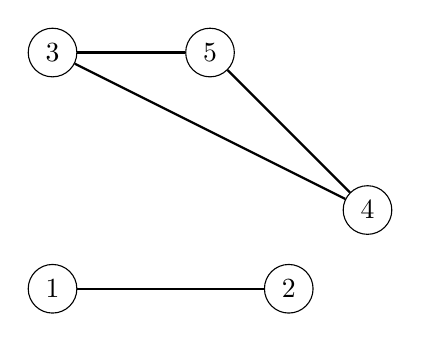
\begin{tikzpicture}
\tikzstyle{vx} = [circle,draw=black] %vertex
\tikzstyle{de} = [-,thick] %directed edge
\node[vx](va)at(0,0){1};
\node[vx](vb)at(3,0){2};
\node[vx](vc)at(0,3){3};
\node[vx](vd)at(4,1){4};
\node[vx](ve)at(2,3){5};
\draw[de](va)--(vb);
\draw[de](vb)--(va);
\draw[de](vc)--(vd);
\draw[de](vd)--(ve);
\draw[de](ve)--(vc);
\end{tikzpicture}
\caption{Solução com subciclos.}\label{fig:PCV subciclos}
\end{subfigure}
\end{figure}

Infelizmente, não existem condições necessárias e suficientes\footnote{Se existissem tais condições, seria possível checá-las para afirmar rapidamente se um grafo tem ciclo hamiltoniano ou não. Se um grafo não satisfizesse as condições necessárias, ele não teria ciclo hamiltoniano; se satisfizesse as condições suficientes, teria. Na ausência destas condições, verificam-se todas as incidências de arestas para fazer esta determinação.} para garantir que um grafo tenha ciclo hamiltoniano. No entanto, existem formulações do PCV feitas para impedir a formação de subciclos. Em uma delas, conhecida como DFJ \cite{DANTZIG:54}, adiciona-se a seguinte família de restrições ao problema:

\begin{equation}
    \sum_{i,j \in S}x_{ij} \leq |S| - 1, \forall S \subsetneq \mcal{V}.
\end{equation}

Para completar um ciclo com $n$ vértices, são necessárias $n$ arestas. Assim, esta família de restrições impede a formação de ciclo hamiltoniano em qualquer subgrafo próprio induzido por vértices do problema. Logo, impede-se a formação de subciclos no grafo do problema. No caso da \cref{fig:PCV laços}, a formação de laços é impedida por todas as restrições da forma $\sum_{i\in S}x_{ii} \leq 0$, com $S = \{i\}$. No caso da \cref{fig:PCV subciclos}, a formação dos dois subciclos é impedida pelas restrições

\begin{align}
\sum_{i,j \in S}x_{ij} \leq 1,\ &S = \{1,2\},\\
\sum_{i,j \in S}x_{ij} \leq 2,\ &S = \{3,4,5\}.
\end{align}

Existem outras formulações populares para o PCV que tentam remover subciclos. Uma delas é a de \textcite{MILLER:60}, conhecida como MTZ, que adiciona ao problema uma variável $u_i$ para cada vértice do PCV. Estas variáveis têm o propósito de ordenar os pontos visitados, respeitando as famílias de restrições

\begin{align}
    &u_i - u_j + nx_{ij} \leq n - 1,\ \forall i \in \mcal{V},\ j \in \mcal{V}\backslash\{0\},\ i \neq j,\\
    &u_i \in \mathbb{Z}.
\end{align}

Se não existir deslocamento de um ponto $i$ a um ponto $j$, então $x_{ij} = 0$ e, consequentemente, sobra que $u_i - u_j \leq n - 1$, o que garante que o valor de cada variável de ordenação não exceda o número de pontos permutáveis do problema. Se existir deslocamento de $i$ a $j$, segue-se que $x_{ij} = 1$ e, desta maneira, $u_i - u_j \leq -1$. Ou seja, o próximo ponto na ordem de deslocamentos deve ficar uma unidade à frente do anterior.

Outra opção é a formulação de \textcite{GAVISH:78}, conhecida como GG, que introduz variáveis de ordenação $z_{ij}$ ao problema, relacionando cada vértice $v_i$ a cada vértice $v_j$. Esta formulação impõe as seguintes famílias de restrições ao problema:

\begin{align}
    &\sum_{j=0}z_{ij} - \sum_{j\neq0}z_{ji} = 1,&i = 1,\ldots,n,\\\label[constraint]{eq:GG1}
    &z_{ij} \leq (n - 1)x_{ij},&i = 1,\ldots,n,\ j = 0,\ldots,n,\\\label[constraint]{eq:GG2}
    &z_{ij} \geq 0,&\forall i, j.
\end{align}

Estas formulações têm diferentes performances quando implementadas em ambiente computacional. Uma discussão detalhada sobre isso é feita na \cref{sec:considerações computacionais}

\begin{exmp}[Complexidade computacional do PCV]
Encontrar a solução ótima de um PCV é algo difícil ou impossível, como descreve Zambito \cite{ZAMBITO:06}. O PCV se enquadra na categoria de problema NP-difícil, o que significa que só é plausível encontrar soluções exatas até certo número de pontos. Para resolver problemas muito grandes, são empregadas técnicas para encontrar soluções próximas da ótima.

A título de ilustração da complexidade do PCV -- e, por extensão, de problemas mais elaborados --, suponha-se o objetivo de determinar a melhor rota de um PCV calculando todas as rotas possíveis e selecionando a que apresentar menor distância total -- ideia que será denominada \emph{método de força bruta}.

Quantas rotas existem em um PCV assimétrico? Os $n$ pontos além do depósito são permutáveis, portanto, existem $n!$ ciclos hamiltonianos possíveis. A distância total de cada ciclo é determinada por $n$ somas de custos de vértice a vértice, o que requer, no mínimo, um total de $n!n$ operações computacionais para que se possa determinar o melhor\footnote{A alocação de memória necessária é um fator que não é contabilizado neste exemplo.}. Supondo tempo de soma individual $\varepsilon$, tem-se os tempos de computação da \cref{tab:computação pcv}.

\begin{table}[H]
\centering
\caption{Fator de aumento do tempo mínimo de computação de um número de pontos para outro no PCV.}\label{tab:computação pcv}
\begin{tabular}{lccS} 
\toprule {Pontos} & {Tempo ($\varepsilon$)} & {Fator de aumento} \\
\midrule 5 &	96 & --\\
  6 & 600	& 6.25\\
 7 & 4320 &	7.2\\
 8 & 35280 & 8.17\\
 9 & 322560 & 9.14\\
 10 & 3265920 & 10.13\\
\bottomrule
\end{tabular}
\end{table}

Nestas condições, um PCV de 10 pontos leva no mínimo 34 mil vezes mais tempo para resolver do que um de 5 pontos. Para um exemplo de implementação e execução do método de força bruta, ver \cite{SIQUEIRA:22}.
\end{exmp}

\subsection{Problemas de otimização}\label{sec:problemas de otimização}
O modelo de PCV simétrico da \cref{sec:PCV} pode ser escrito como

\begin{align}
    \min &\sum_{i,j \in \mcal{V}}{x_{ij}c_{ij}},&\label[expression]{eq:PCV min}\\
    \text{s.a } &\sum_{j \in \mcal{V}}x_{ij} = 2,\ &\forall i \in \mcal{V},\label[constraints]{eq:PCV restrição simétrica}\\
    &\sum_{i,j \in S}x_{ij} \leq |S| - 1,\ &\forall S \subsetneq \mcal{V},\label[constraints]{eq:PCV subciclos}\\
    &x_{ij} \in \{0,1\},\ &\forall i, j \in \mcal{V}.\label[constraints]{eq:PCV binário}
\end{align}

A \cref{eq:PCV min} define o PCV como um problema de \emph{minimização}, o que o coloca na categoria de problema de \emph{otimização}\footnote{Outra palavra muito utilizada para se referir a otimização é \emph{programação}. Preferimos evitar o uso deste termo devido à possibilidade de confusão com programação de computadores.}. Considerando-se as \cref{eq:PCV restrição simétrica,eq:PCV subciclos}, tem-se um problema de otimização \emph{linear}. Este tipo de problema aparece na \emph{forma padrão}

\begin{align}\label[problem]{eq:forma padrão}
    \min\ & z \coloneqq \objval\\
    \textrm{s.a }& Ax \leq b,\\
    &x \geq \vb{0},
\end{align}
em que $c \in \mathbb{R}^n$ é o vetor de coeficientes de custo, $x \in \mathbb{R}^n$ é o vetor de variáveis de decisão, $A \in \mathbb{R}^{m\times n}$ é a matriz de coeficientes de restrições e $b \in \mathbb{R}^m$ é o vetor do lado direito das inequações do problema. Chama-se $z$ de \emph{valor objetivo} ou \emph{função objetivo}. Em geral, é desejável ter $b \geq \vb{0}$. Assim, para todo elemento $b_i \leq 0$, multiplica-se a inequação $A_ix \leq b_i$ por $-1$, invertendo o sinal da inequação.

A \emph{forma canônica} de um problema de otimização linear é

\begin{align}
    \min\ & z \coloneqq \objval\label{eq:OL}\tag{OL}\\
    \textrm{s.a }& Ax = b,\\
    &x \geq \vb{0}.
\end{align}

Para converter um problema para a forma canônica, adicionam-se ou subtraem-se variáveis não-negativas de todas as inequações, transformando-as em equações. Tais variáveis são chamadas de \emph{variáveis de folga}.

\begin{itemize}
    \item Se $A_ix \leq b$, então adiciona-se $x_s \geq 0$ tal que $A_ix + x_s = b_i$;
    \item Se $A_ix \geq b$, então subtrai-se $x_s \geq 0$ tal que $A_ix - x_s = b_i$. 
\end{itemize}

A conversão para a forma canônica é feita para possibilitar sua resolução pelo método simplex. Este método foi desenvolvido pelo matemático George Dantzig na década de 40. Os avanços em computação financiados pelo departamento de defesa dos Estados Unidos na época incentivaram as pesquisas de Dantzig e outros matemáticos \cite{DANTZIG:90}. As pesquisas em otimização linear renderam frutos em várias indústrias e processos logísticos, sendo cruciais no campo da pesquisa operacional \cite{SOBRAPO:17}.

Apesar da sua grande utilidade, o método simplex se limita a resolver problemas de otimização linear. Como dito no começo desta seção, o PCV só é linear quando as \cref{eq:PCV binário} são desconsideradas. Este tipo de técnica, em que restrições que forçam variáveis a serem inteiras são descartadas, é chamado de \emph{relaxação} do problema \cite{BEASLEY}.

Quando o modelo completo do PCV é considerado, tem-se um problema de otimização \emph{inteira}, dado que todas as variáveis de decisão são inteiras. Para problemas mais complexos, é possível fazer uma mistura de variáveis inteiras com variáveis reais, o que categoriza um problema de otimização \emph{inteira mista} \cite{LAVROV:19,KARVE:22,BRIDGELALL:22}.

A álgebra linear desenvolvida no restante desta seção é necessária para compreender os alicerces do método simplex e as implementações computacionais realizadas neste trabalho. Para uma explicação sobre os procedimentos do simplex, consultar o \cref{sec:metodo_simplex}.

\subsection{Poliedros e convexidade}

\begin{mydef}[Poliedro] \label{def:poliedro}
Um \emph{poliedro} $\vb P$ é um conjunto que pode ser escrito na forma $\vb P \coloneqq \{x \in \mathbb{R}^n \mid Ax \leq b\}$, onde $A$ é uma matriz $m\times n$ e $b$ é um vetor em $\mathbb{R}^m$.
\end{mydef}

O conjunto de restrições que definem um problema de otimização linear \eqref{eq:OL} pode ser interpretado como um poliedro. Esta interpretação geométrica facilita a compreensão dos problemas. É possível interpretar as próprias restrições como objetos geométricos, sendo o poliedro o resultado da intersecção destes objetos. Assim, todo ponto que satisfizer todas as restrições do poliedro é dito \emph{factível} \cite{LEWIS:08}.

\begin{mydef}[Hiperplano] \label{def:hiperplano}
 Seja $a$ um vetor não-nulo em $\mathbb{R}^n$ e seja $b$ um escalar. Então o conjunto $\vb H \coloneqq \{x \in \mathbb{R}^n \mid a^\intercal x = b\}$ é chamado de \emph{hiperplano}.
\end{mydef}

\begin{mydef}[Semiespaço] \label{def:semiespaço}
 Seja $a$ um vetor não-nulo em $\mathbb{R}^n$ e seja $b$ um escalar. Então o conjunto $\vb S \coloneqq \{x \in \mathbb{R}^n \mid a^\intercal x \leq b\}$ é chamado de \emph{semiespaço}.
\end{mydef}

Hiperplanos e semiespaços são generalizações dos conceitos tridimensionais de aresta e espaço. Um exemplo visual destes conceitos é apresentado na \cref{fig:semiespaço e hiperplano}. O plano em azul transparente é um semiespaço definido por uma desigualdade $a^\intercal x \leq b$, enquanto o hiperplano é a reta que delimita este semiespaço na igualdade $a^\intercal x = b$.

\begin{figure}
    \centering
    \captionof{figure}{Exemplo de hiperplano ($\mcal{H}$) e semiespaço ($\mcal{S}$)}\label{fig:semiespaço e hiperplano}
    \begin{overpic}[scale=0.5]{imagens/semiespaço.pdf}
    \put(55, 33){\huge$\mcal{H}$}
    \put(20, 20){\huge$\mcal{S}$}
    \end{overpic}
\end{figure}

A convexidade é uma propriedade fundamental para poliedros passíveis de resolução pelo método simplex. A seguir, são apresentados alguns conceitos e teoremas a respeito desta propriedade.

\begin{mydef}[Conjunto convexo] \label{def:conjunto_convexo}
 Um conjunto $\vb S\subset \mathbb{R}^n$ é \emph{convexo} se, para todo $x, y \in \vb S$, e qualquer $\lambda \in [0,1]$, tem-se $\lambda x + (1-\lambda) y \in \vb S$.
\end{mydef}

\begin{mydef}[Combinação convexa e envoltória convexa] \label{def:combinação_e_casco_convexo}
 Sejam $x^1, \ldots, x^k$ vetores em $\mathbb{R}^n$ e sejam $\lambda_1, \ldots, \lambda_n$ escalares não-negativos cuja soma é um. Então:
 \begin{enumerate}[(a)]
     \item O vetor $\sum^k_{i=1}\lambda_i x^i$ é uma \emph{combinação convexa} dos vetores $x^1, \ldots, x^k$.
     \item A \emph{envoltória convexa} dos vetores $x^1, \ldots, x^k$ é o conjunto de todas as combinações convexas desses vetores.
 \end{enumerate}
\end{mydef}

\begin{theorem} \label{teo:conjuntos_convexidade}
 \begin{enumerate}[(a)]
     \item \label{item:convexos_a} A intersecção de conjuntos convexos é convexa.
     \item Todo poliedro é um conjunto convexo.
     \item Uma combinação convexa de um número finito de elementos de um conjunto convexo pertence ao conjunto convexo.
     \item A envoltória convexa de um número finito de vetores é um conjunto convexo.
 \end{enumerate}
\end{theorem}

\begin{proof}
 \begin{enumerate}[(a)]
     \item\label{item:convexo_a} Sejam $\vb{S_i}, i \in I$ conjuntos convexos onde $I$ é um conjunto de índices, e suponha que $x$ e $y$ pertencem à intersecção $\cap _{i\in I}\vb{S_i}$. Seja $\lambda\in [0,1]$. Como cada $\vb{S_i}$ é convexo e contém $x$ e $y$, temos $\lambda x + (1 - \lambda)y \in \vb{S_i}$, o que prova que $\lambda x + (1-\lambda)y$ também pertence à intersecção dos conjuntos $\vb{S_i}$. Logo, $\cap _{i \in I} \vb{S_i}$ é convexo.
     \item Sejam $a$ um vetor e $b$ um escalar. Suponha que $x$ e $y$ satisfazem $a^\intercal x\leq b$ e $a^\intercal y\leq b$, respectivamente, e logo pertencem ao mesmo semiespaço. Seja $\lambda \in [0,1]$. Então $a^\intercal(\lambda x + (1-\lambda)y)\leq \lambda b + (1-\lambda)b = b$, o que prova que $\lambda x + (1 - \lambda)y$ também pertence ao mesmo semiespaço. Logo, um semiespaço é convexo. Como um poliedro é uma intersecção de um número finito de semiespaços, o resultado é confirmado pelo \cref{item:convexo_a}.
     \item Uma combinação convexa de dois elementos de um conjunto convexo está contida no conjunto, pela definição de convexidade. Suponhamos, por hipótese indutiva, que uma combinação convexa de $k$ elementos de um conjunto convexo pertence ao conjunto. Considere $k+1$ elementos $x^1,\ldots,x^{k+1}$ de um conjunto convexo $\vb S$ e sejam $\lambda_1,\ldots,\lambda_{k+1}$ escalares não-negativos de soma um. Assumimos, sem perda de generalidade, que $\lambda_{k+1}\neq1$. Então temos:
     
     \begin{equation}\label{item:convexo_c}
        \sum^{k+1}_{i=1}\lambda_ix^i=\lambda_{k+1}x^{k+1}+(1-\lambda_{k+1})\sum^k_{i=1}\frac{\lambda_i}{1-\lambda_{k+1}}x^i.
    \end{equation}
    
    Note que $\sum_{i=1}^k{\frac{\lambda_i}{1-\lambda_{k+1}}} = 1$, pois, como definido anteriormente, $\sum_{i=1}^{k+1}{\lambda_i} = 1$, o que implica que $(\sum_{i=1}^{k+1}\lambda_i) - \lambda_{k+1} = 1 - \lambda_{k+1} = \sum_{i=1}^{k}\lambda_i$. Usando a hipótese indutiva, $\sum^k_{i=1}\frac{\lambda_{i}x^i}{1-\lambda_{k+1}} \in \vb S$. Então, o fato de $\vb S$ ser convexo e a \cref{item:convexo_c} implicam que $\sum^{k+1}_{i=1}\lambda_ix^i\in \vb S$, e a indução está completa.
     \item Seja $\vb S$ a envoltória convexa dos vetores $x^1,\ldots,x^k$, e sejam $y=\sum^k_{i=1}\xi_ix^i,z=\sum^k_{i=1}\theta_ix^i$ dois elementos de $\vb S$, onde $\xi_i\geq0, \theta_i\geq0$ e $\sum^k_{i=1}\xi_i=\sum^k_{i=1}\theta_i=1$. Seja $\lambda\in[0,1]$. Então, $\lambda y + (1-\lambda)z=\lambda\sum^k_{i=1}\xi_ix^i+(1-\lambda)\sum^k_{i=1}\theta_ix^i=\sum^k_{i=1}(\lambda\xi_i+(1-\lambda)\theta_i)x^i$.
     
     Note que os coeficientes $\lambda\xi_i+(1-\lambda)\theta_i, i=1,\ldots,k$ são não-negativos e somam um. Isso mostra que $\lambda y + (1-\lambda)z$ é uma combinação convexa de $x^1,\ldots,x^k$ e, portanto, pertence a $\vb S$. Isso estabelece a convexidade de $\vb S$.
 \end{enumerate}
\end{proof}

\subsection{Ponto extremo e vértice}\label{sec:ponto extremo e vértice}
Os conceitos de ponto extremo e vértice são fundamentais em otimização linear. Como é provado na \cref{sec:equivalências}, estes conceitos são equivalentes entre si, além de serem equivalentes ao conceito de solução básica factível, introduzido na \cref{sec:sbf}. Como é provado no \cref{sec:simplex pontos extremos}, a solução ótima de um problema com restrições lineares se encontra sempre em um de seus vértices, quando o poliedro do problema é limitado.

\begin{mydef}[Ponto extremo]
 Seja $\vb P$ um poliedro. Um vetor $x\in \vb P$ é um \emph{ponto extremo} de $\vb P$ se não existem dois vetores $y, z\in \vb P$, ambos diferentes de $x$, e um escalar $\lambda\in[0,1]$, tais que $x=\lambda y+(1-\lambda)z$.
\end{mydef}

Uma interpretação possível de pontos extremos pode ser obtida desenhando a ponta de um poliedro e seus arredores.

\begin{figure}[H]
\centering
\caption{Exemplo visual de ponto extremo}\label{fig:exemplo_poliedro}
   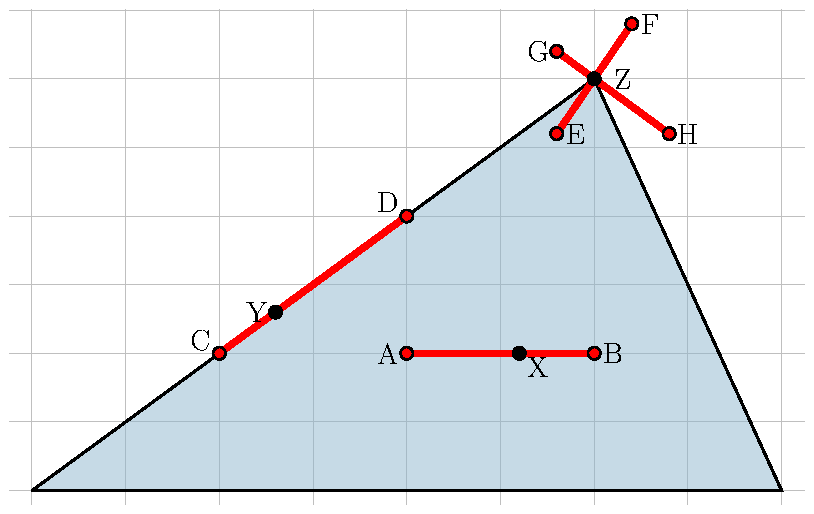
\includegraphics[scale=1]{imagens/pontos_extremos.pdf}
\end{figure}

O exemplo da \Cref{fig:exemplo_poliedro} possui um poliedro, em azul, três pontos pretos que se espera representar por combinação convexa e quatro combinações de pontos, em vermelho. O ponto $X$ pode ser representado por combinação convexa dos pontos $A$ e $B$, pois ambos se encontram dentro do poliedro. O ponto $Y$, localizado numa das arestas do poliedro, também pode ser representado por combinação convexa de dois pontos, neste caso $C$ e $D$, ambos localizados na mesma aresta que $Y$.

O que não podemos representar por combinação convexa de dois pontos é o ponto $Z$, que se localiza justamente numa das pontas do poliedro. As únicas combinações cujos segmentos de reta resultantes passam por $Z$ contêm um ponto dentro e outro fora do poliedro ($E$ e $F$, por exemplo) ou dois pontos fora do poliedro ($G$ e $H$, por exemplo). Portanto, dos três pontos pretos, apenas $Z$ não pode ser representado como combinação convexa, e, logo, ele é um ponto extremo.

\begin{mydef}[Vértice]\label{def:vértice}
 Seja $\vb P$ um poliedro. Um vetor $x\in \vb P$ é um \emph{vértice} de $\vb P$ se existir vetor $c$ tal que $c^\intercal x < c^\intercal y$ para qualquer $y$ que satisfaça $y\in \vb P$ e $y\neq x$.
\end{mydef}

Geometricamente, os vértices podem ser percebidos conforme a \Cref{fig:vertices}.

\begin{figure}[H]
\centering
\caption{Exemplo visual de vértice}\label{fig:vertices}
   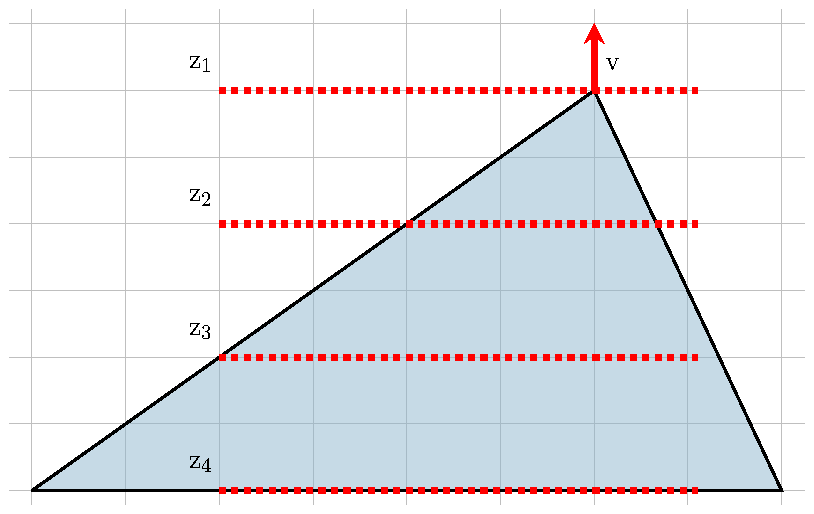
\includegraphics[scale=1]{imagens/vertice.pdf}
\end{figure}

O vetor $v$ define infinitos hiperplanos cujos valores crescem no sentido do vetor. O conjunto desses hiperplanos define um semiespaço. Desta maneira, temos que $z_1 > z_2 > z_3 > z_4$. Perceba que os valores $z_2$, $z_3$ e $z_4$ podem ser obtidos multiplicando $v$ por infinitos pontos do poliedro, justamente os que estão nas linhas tracejadas que representam os respectivos hiperplanos. Escolhemos um de cada, que denotaremos pelos vetores $x^2$, $x^3$ e $x^4$. Ou seja, $v^\intercal x^2 = z_2$, $v^\intercal x^3 = z_3$ e $v^\intercal x^4 = z_4$. No entanto, existe um único vetor do poliedro através do qual se pode obter $z_1$, que é o vetor que descreve a sua ponta, $x^1$. Portanto, existe um único ponto do poliedro cujo produto interno com o vetor $v$ é maior do que seu produto interno com qualquer outro ponto do poliedro, e, então, este ponto só pode ser um vértice.

\subsection{Solução básica factível}\label{sec:sbf}
\begin{mydef}[Espaço vetorial]
 Um \emph{espaço vetorial} é um conjunto cujos elementos, chamados vetores, podem ser somados e multiplicados por números escalares.
\end{mydef}

\begin{mydef}[Subespaço]
 Um subconjunto não-vazio $\vb S$ de $\mathbb{R}^n$ é chamado de \emph{subespaço} de $\mathbb{R}^n$ se $ax + by \in S$ para todo $x, y \in \vb S$ e todo $a, b \in \mathbb{R}$. Se $\vb S\neq\mathbb{R}^n$, $\vb S$ é um \emph{subespaço próprio}. Todo subespaço precisa conter o vetor nulo.
\end{mydef}

\begin{mydef}[Espaço gerado]
 O \emph{espaço gerado (span)} de um número finito de vetores $x^1,\ldots,x^K$ em $\mathbb{R}^n$ é um subespaço de $\mathbb{R}^n$ definido como o conjunto de todos os vetores $y$ da forma $y=\sum^K_{k=1}a_kx^k$, onde cada $a_k$ é um número real. Qualquer vetor $y$ assim é chamado de \emph{combinação linear} de $x^1,\ldots,x^K$.
\end{mydef}

\begin{mydef}[Base]
 Dado um subespaço $\vb S$ de $\mathbb{R}^n$, com $\vb S\neq\{0\}$, uma \emph{base} de $\vb S$ é uma coleção de vetores que são linearmente independentes e cujo espaço gerado é igual a $\vb S$. Toda base de um subespaço tem o mesmo número de vetores, que é chamado de \emph{dimensão} do subespaço. Em particular, a dimensão de $\mathbb{R}^n$ é $n$, e todo subespaço próprio de $\mathbb{R}^n$ tem uma dimensão menor do que $n$.
\end{mydef}

\begin{mydef}[Subespaço afim]
Seja $\vb{S_0}$ um subespaço de $\mathbb{R}^n$ e seja $x^0$ algum vetor. O vetor $\vb S$ definido como

$$\vb S = x^0 + \vb{S_0} = \{x + x^0 \mid x \in \vb{S_0}\}$$
é chamado de \emph{subespaço afim}, e corresponde a uma translação do subespaço $\vb{S_0}$. Por definição, a dimensão de $\vb S$ é igual à dimensão de $\vb{S_0}$.
\end{mydef}

\begin{theorem}\label{teo:base}
Suponha que o espaço gerado $\vb S$ dos vetores $x^1,\ldots,x^K$ tem dimensão $m$. Então:
\begin{enumerate}[(a)]
\item Existe uma base de $\vb S$ consistindo de $m$ dos vetores $x^1,\ldots,x^K$.
\item Se $k\leq m$ e $x^1,\ldots,x^k$ são linearmente independentes, podemos formar uma base de $\vb S$ começando com $x^1,\ldots,x^k$ e escolhendo $m-k$ dos vetores $x^{k+1},\ldots,x^K$.
\end{enumerate}
\end{theorem}

\begin{proof}
Vamos começar provando o teorema pelo item (b). A princípio, se todos os vetores $x^{k+1},\ldots,x^K$ puderem ser representados como combinações lineares dos vetores $x^1,\ldots,x^k$, então os vetores $x^1,\ldots,x^k$ formam uma base do subespaço e, portanto, ${k = m}$. Do contrário, podemos encontrar um vetor em $x^{k+1},\ldots,x^K$ que seja linearmente independente de todos os vetores em $x^1,\ldots,x^k$, aumentando para k + 1 o número de vetores linearmente independentes. Repetindo este processo $m - k$ vezes, obtemos a base desejada de $\vb S$. O item (a) decorre trivialmente do caso em que começamos com $k = 0$ no processo que acabamos de apresentar.
\end{proof}

Com estas definições, podemos retornar aos pontos extremos e aos vértices. O fato é que as definições desses dois conceitos são de difícil implementação computacional. No caso de pontos extremos, precisaríamos encontrar uma forma de garantir ao computador que nenhuma de uma infinidade de possíveis combinações de dois pontos é igual ao ponto que se deseja provar extremo. Já no caso de vértices, há uma infinidade de vetores passíveis de teste.

Para contornar este problema, introduziremos a definição algébrica de soluções básicas factíveis. Para tal, primeiro vamos considerar um poliedro $\vb P \subset \mathbb{R}^n$ definido em termos de restrições de igualdade e desigualdade:

\begin{equation}
\begin{aligned}
 &a_i^\intercal x\geq b_i,\quad i \in \vb{M_1},\nonumber\\
 &a_i^\intercal x\leq b_i,\quad i \in \vb{M_2},\nonumber\\
 &a_i^\intercal x = b_i,\quad i \in \vb{M_3}.\nonumber
\end{aligned}
\end{equation}

Em que $\vb{M_1, M_2}$ e $\vb{M_3}$ são conjuntos finitos de índices, cada $a_i$ é um vetor em $\mathbb{R}^n$, e cada $b_i$ é um escalar.

\begin{mydef}[Restrição ativa]
 Se um vetor $x^*$ satisfaz $a^\intercal _ix^*=b_i$ para algum $i$ em $\vb{M_1, M_2}$ ou $\vb{M_3}$, dizemos que a restrição correspondente é \emph{ativa} (\emph{active} ou \emph{binding}) em $x^*$.
\end{mydef}

Se existirem $n$ restrições que são ativas em um vetor $x^*$, então $x^*$ satisfaz um certo sistema de $n$ equações lineares com $n$ incógnitas. Este sistema só terá solução única se as $n$ equações forem linearmente independentes. Disso, segue o teorema:

\begin{theorem}\label{teo:af_eq}
Seja $x^*$ um elemento de $\mathbb{R}^n$ e seja $I(x^*) = \{i \mid a_i^\intercal x = b_i\}$ o conjunto dos índices das restrições que são ativas em $x^*$. Então as seguintes afirmações são equivalentes:
\begin{enumerate}[(a)]
\item\label{item:ativa_a} Existem $n$ vetores no conjunto $\{a_i\mid i\in I\}$, que são linearmente independentes.
\item\label{item:ativa_b} O espaço gerado dos vetores $a_i, i\in I$ é todo o $\mathbb{R}^n$; ou seja, todo elemento de $\mathbb{R}^n$ pode ser expresso como uma combinação linear dos vetores $a_i, i\in I$.
\item\label{item:ativa_c} O sistema de equações $a^\intercal _ix = b_i, i \in I$ tem uma única solução.
\end{enumerate}
\end{theorem}

\begin{proof}
Suponha que os vetores $a_i, i\in I$ gerem o espaço $\mathbb{R}^n$. Então, o espaço gerado desses vetores tem dimensão $n$. Pelo \cref{teo:base}, $n$ desses vetores formam uma base de $\mathbb{R}^n$ e são, portanto, linearmente independentes. Por outro lado, suponha que $n$ dos vetores $a_i, i\in I$ são linearmente independentes. Então, o subespaço gerado por esses $n$ vetores é n-dimensional e precisa ser igual a $\mathbb{R}^n$. Logo, todo elemento de $\mathbb{R}^n$ é uma combinação linear dos vetores $a_i, i \in I$. Isso estabelece a equivalência do \cref{item:ativa_a} e do \cref{item:ativa_b}.

Se o sistema de equações tem múltiplas soluções -- por exemplo, $x^1$ e $x^2$ -- então o vetor não-nulo $d = x^1 - x^2$ satisfaz $a_i^\intercal d = 0$ para todo $i\in I$. Como $d$ é ortogonal a todo $a_i, i\in I$, $d$ não é uma combinação linear desses vetores e logo os vetores $a_i, i\in I$ não geram $\mathbb{R}^n$. Reciprocamente, se os vetores $a_i, i \in I$ não geram $\mathbb{R}^n$,  escolhemos um vetor não-nulo $d$ que seja ortogonal ao subespaço gerado por esses vetores. Se $x$ satisfaz $a_i^\intercal x = b_i$ para todo $i\in I$, também temos $a^\intercal _i(x+d)=b_i$ para todo $i\in I$, obtendo, assim, várias soluções. Logo, estabelecemos a equivalência entre o \cref{item:ativa_b} e o \cref{item:ativa_c}.
\end{proof}

A partir daqui, faremos um abuso de linguagem e diremos que uma restrição será linearmente independente quando seu vetor $a_i$ for linearmente independente dos vetores $a_i$ das demais restrições.

\begin{mydef}[Solução básica e solução básica factível]\label{def:sbf}
 Considere um poliedro $\vb P$ definido por restrições lineares de igualdade e desigualdade, e seja $x^*$ um elemento de $\mathbb{R}^n$.
 \begin{itemize}
 \item O vetor $x^*$ é uma \emph{solução básica} se todas as restrições de igualdade são ativas nele e se, de todas as restrições ativas em $x^*$, existem $n$ que são linearmente independentes.
 \item Se $x^*$ é uma solução básica que satisfaz todas as restrições do poliedro, ela é uma \emph{solução básica factível}.
\end{itemize}
\end{mydef}

Como explicado no \cref{sec:metodo_simplex}, o método simplex "salta" de uma solução básica factível a outra de maneira condizente com a definição a seguir.

\begin{mydef}[Soluções básicas adjacentes]
    Duas soluções básicas distintas no $\mathbb{R}^n$ são \emph{adjacentes} quando existem $n - 1$ restrições linearmente independentes que são ativas em ambas.
\end{mydef}

Além disso, outra definição que será importante é a de \emph{degeneração}.

\begin{mydef}[Degeneração]\label{def:degeneração}
    Uma solução básica $x \in \mathbb{R}^n$ é \emph{degenerada} se mais do que $n$ restrições são ativas em $x$.
\end{mydef}

Por fim, uma última observação importante a ser feita sobre soluções básicas factíveis é o teorema a seguir.

\begin{theorem}\label{teo:SBFs finitas}
Para um número finito de restrições lineares de desigualdade, só pode existir um número finito de soluções básicas.
\end{theorem}
\begin{proof}
    Considere um sistema de $m$ restrições lineares de desigualdade impostas a um vetor $x \in \mathbb{R}^n$. Em qualquer solução básica, existem $n$ restrições linearmente independentes ativas. Pelo \cref{teo:af_eq}, estas $n$ restrições linearmente independentes definem um ponto único. Logo, diferentes soluções básicas correspondem a diferentes combinações de $n$ restrições linearmente independentes ativas e, portanto, correspondem a diferentes pontos únicos. Assim sendo, o número de soluções básicas é limitado pela quantidade de combinações possíveis de $n$ restrições linearmente independentes de um total de $m$.
\end{proof}

Assim, como diz Santos \cite{LRSANTOS:14}, o número máximo possível de soluções básicas factíveis para um problema é a permutação
\begin{equation}\label{eq:maxSBF}
    \binom{n}{m} = \frac{n!}{m!(n-m)!} \geq \left(\frac{n}{m}\right)^m,
\end{equation}
o que evidencia que o número de soluções básicas e básicas factíveis de um problema cresce rapidamente conforme são adicionadas restrições e variáveis.

\subsection{Equivalências}\label{sec:equivalências}

\begin{theorem}
Seja $\vb P$ um poliedro não-vazio e seja $x^*\in \vb P$. Então, as seguintes afirmações são equivalentes:
\begin{enumerate}[(i)]
\item $x^*$ é um vértice;
\item $x^*$ é um ponto extremo;
\item $x^*$ é uma solução básica factível.
\end{enumerate}
\end{theorem}

\begin{proof}
Para os propósitos desta prova, e sem perda de generalidade, assumiremos que $\vb P$ é representado em termos de restrições da forma $a_i^\intercal x \leq b_i$ e $a_i^\intercal x = b_i$.

\textbf{Vértice} $\Rightarrow$ \textbf{Ponto Extremo}

Suponha que $x^*\in \vb P$ é um vértice. Pela \cref{def:vértice}, existe algum $c \in \mathbb{R}^n$ tal que $c^\intercal x^* < c^\intercal y$ para todo $y\in \vb P$ tal que $y\neq x^*$. Se $w\in \vb P, z\in \vb P, w\neq x^*, z\neq x^*$ e $0\leq\lambda\leq1$, então, $c^\intercal x^* < c^\intercal w, c^\intercal x^*<c^\intercal z$, o que implica que $c^{T} x^{*} < c^\intercal (\lambda w + (1-\lambda)z)$ e, portanto, $x^*\neq \lambda w + (1-\lambda) z$. Logo, $x^*$ não pode ser representado como combinação convexa de dois outros elementos de $\vb P$ e, portanto, é um ponto extremo.

\textbf{Ponto Extremo} $\Rightarrow$ \textbf{Solução Básica Factível}

Suponha que $x^*\in \vb P$ não é uma solução básica factível. Mostraremos que $x^*$ não é ponto extremo de $\vb P$. Seja $I = \{i\mid a_i^\intercal x=b_i\}$. Como $x^*$ não é solução básica factível, não existem $n$ vetores linearmente independentes na família $a_i, i\in I$, pois, se existissem, $x^*$ teria que estar fora do poliedro e, assim, não faria sentido considerá-lo. Logo, os vetores $a_i, i \in I$ estão em um subespaço do $\mathbb{R}^n$, e existe um vetor não-nulo $d \in \mathbb{R}^n$ tal que $a_i^\intercal d = 0$, para todo $i \in I$.

Seja $\epsilon$ um número positivo pequeno e considere os vetores $y = x^* + \epsilon d$ e $z = x^* - \epsilon d$. Perceba que $a_i^\intercal y = a_i^\intercal z = a_i^\intercal x^* = b_i$, para $i\in I$. Ademais, para $i\not\in I$, temos $a_i^\intercal x^*<b_i$ e, dado que $\epsilon$ é pequeno, também temos $a_i^\intercal y<b_i$. Logo, quando $\epsilon$ é suficientemente pequeno, $y\in P$ e, por argumento similar, $z\in P$. Por fim, note que $x^* = \frac{y+z}{2}$, o que implica que $x^*$ não é ponto extremo.

\textbf{Solução Básica Factível} $\Rightarrow$ \textbf{Vértice}

Seja $x^*$ uma solução básica factível e seja $I = \{i\mid a_i^\intercal x^*=b_i\}$. Seja $c = \sum_{i\in I}a_i$. Então temos

\begin{equation}c^\intercal x^* = \sum_{i\in I}a_i^\intercal x^*=\sum_{i\in I}b_i.
\end{equation}

Ademais, para todo $x\in P$ e todo $i$, temos $a_i^\intercal x\leq b_i$, e

\begin{equation}
c^\intercal x = \sum_{i\in I}a_i^\intercal x\leq \sum_{i\in I} b_i.\label{eqn:c}
\end{equation}

Isso mostra que $x^*$ é uma solução ótima para o problema de minimizar $c^\intercal x$ no conjunto $\vb P$. Ademais, a igualdade é possível na \cref{eqn:c} se e somente se $a_i^\intercal x = b_i$, para todo $i \in I$. Como $x^*$ é uma solução básica factível, existem $n$ restrições linearmente independentes que são ativas em $x^*$, e $x^*$ é solução única para o sistema de equações $a_i^\intercal x = b_i, i \in I$ (\cref{teo:af_eq}). Logo, $x^*$ é o minimizador único de $c^\intercal x$ no conjunto $\vb P$ e, portanto, é um vértice de $\vb P$.
\end{proof}

\subsection{Resumo do método simplex}
Nesta seção, é apresentado um resumo do \cref{sec:metodo_simplex}.

Todo problema de otimização linear em cujo poliedro exista pelo menos um ponto possui solução. Quando o poliedro é limitado (isto é, quando não existe semirreta contida no poliedro), a solução ótima para o problema está, necessariamente, localizada em algum dos seus vértices. Nos casos em que o poliedro é ilimitado, além de poder estar em um vértice, a solução ótima pode ser $-\infty$ ou $\infty$ (para problemas de minimização e maximização, respectivamente). Nestes dois últimos casos, não existe ponto específico que otimize a função objetivo.

O método simplex funciona baseado nestes conhecimentos. Assumindo que a matriz de restrições de um problema tenha posto completo, pode-se resumir o método da seguinte maneira:

\begin{enumerate}[(a)]
    \item Encontra-se um vértice do poliedro do problema, se existir;\label{it:simplex_a}
    \item Analisam-se os vértices adjacentes ao atual:\label{it:simplex_b}
    \begin{enumerate}[1.]
        \item Se não existir vértice que reduza o valor objetivo, pular para (c);
        \item Do contrário, mover-se para o vértice que reduza ao máximo o valor objetivo e repetir (b).
    \end{enumerate}
    \item Verificam-se as variáveis de decisão do problema:
    \begin{enumerate}[1.]
        \item Se existir variável que possa ser aumentada infinitamente, sem violar a factibilidade do poliedro, a solução ótima é $\infty$ ou $-\infty$;
        \item Do contrário, a solução ótima se encontra no vértice atual.
    \end{enumerate}
\end{enumerate}

Um empecilho ao \cref{it:simplex_a} é a dificuldade de obtenção de um vértice inicial. A \cref{eq:maxSBF} deixa claro que o número de soluções básicas cresce rapidamente com a complexidade do problema tratado, de modo que determinar um vértice inicial por tentativa e erro possa ser ineficiente. O método para encontrar vértices iniciais implementado neste trabalho é o \emph{método das duas fases}, que resolve um novo problema, cujo vértice inicial é conhecido, e cuja solução ótima é um vértice do problema original. Quando um vértice inicial não é encontrado, o problema não tem solução factível.

A degeneração é um problema que afeta o \cref{it:simplex_b}. Ao encontrar um vértice degenerado, é possível que o simplex entre em um laço infinito em que permaneça no mesmo vértice. Assim como no caso anterior, existem várias formas de resolver este problema. Para propósitos acadêmicos, a \emph{regra lexicográfica} implementada neste trabalho é satisfatória.

Apesar de o método simplex resolver apenas problemas de otimização linear, existem técnicas que permitem que problemas de otimização inteira e inteira mista sejam resolvidos com a ajuda do simplex.